% !TeX program = xelatex
% ============================================================
% 2022 C 题  问题一前半（1a）：表面风化与类型、纹饰、颜色的关联分析
% 简化版（分层列联主线）；高级方法复核版备份在 p1a_paper_q1a_v1_advanced.tex
% 图表文件位于 p1a_out/；全部数值由 p1a_main.py（种子 2026）产生，
% 以 p1a_out/p1a_run_log.txt 为准
% 编译：xelatex p1a_paper_q1a.tex（需 ctex、booktabs，跑两遍）
% ============================================================
\documentclass[12pt]{ctexart}
\usepackage[a4paper,margin=2.5cm]{geometry}
\usepackage{booktabs}
\usepackage{graphicx}
\usepackage{amsmath,amssymb}
\usepackage{caption}
\usepackage{float}
\graphicspath{{p1a_out/}}
\captionsetup{font=small}

\begin{document}

\section{表面风化与玻璃类型、纹饰、颜色的关联分析}

\subsection{问题分析与建模思路}

本节基于附件表单~1 的 58 条文物级记录，分析表面风化与玻璃类型、纹饰、颜色三个分类属性的关系，其中类型含高钾 18 件与铅钡 40 件，纹饰含 A 档 22 件、B 档 6 件、C 档 30 件，颜色 8 类中 4 件缺失，风化 34 件对无风化 24 件。该子问题的产出是关联结论及其证据强度，而非预测模型；化学成分数据留待本问题后半部分使用。

对三个属性逐一做两两检验后直接下结论并不可靠。表单~2 的采样点名称提示风化同时存在文物级与点级两个层次，而更直接的原因是三个属性自身并不独立：下文的纠缠诊断将给出，类型与纹饰的关联系数达到 0.51。若逐一比较，类型与风化的关系会渗入纹饰、颜色的估计，反之亦然。为此本文按三个递进的问题组织分析：第一，每个属性各自与风化有没有关系，以精确检验与置换检验回答；第二，属性间的纠缠是否掩盖或夸大了这些关系，以关联系数诊断加按类型分层回答；第三，结论对样本扰动与口径选择是否稳健，以 Bootstrap 与口径对照回答。三个问题的答案在 1.7 节并排对照，联合考虑相对单独考虑的收益以数值呈现。

\subsection{模型假设}

\textbf{假设 1（标签一致性）}\ 每件文物的表面风化标签对其名下全部采样点成立。核查依据：表单~2 的 69 个采样点中，带未风化点或严重风化点后缀且属于无风化文物的点为 0 个。排除项：不考虑风化层内部的程度差异，该差异交由本问题后半的成分分析处理。目的：保证底表中每个计数单元的归属唯一。

\textbf{假设 2（随机抽样）}\ 58 件文物是来自所研究古代玻璃总体的独立随机样本。排除项：不考虑同墓共出或同批工艺造成的文物间相关性，附件未提供批次信息，该相关性无法度量。目的：保证各检验的独立性前提。

\textbf{假设 3（缺失机制）}\ 4 件颜色缺失文物（编号 19、40、48、58）按单列的未记录类参与统计而非随机填补。事实依据：4 件全部为风化状态的铅钡玻璃，颜色缺失与风化相关而与类型、纹饰无必然联系，随机填补会把颜色不可辨认误计为某个真实色系。目的：保持列联计数的口径干净。

\textbf{设计说明}\ 假设~2 若不成立，各检验的 $p$ 值将系统性偏乐观。本文的对策是以效应量为主、$p$ 值为辅：类型与风化的关联同时给出 $OR=4.67$ 与 $V=0.34$，两者不依赖 $p$ 值的渐近性质；1.8 节的重抽样与口径敏感性检查进一步量化结论对样本扰动的敏感程度。

\subsection{符号说明}

\begin{table}[H]
\centering
\caption{主要符号}
\begin{tabular}{cl}
\toprule
符号 & 含义 \\
\midrule
$n$ & 样本量，本文 $n=58$（涉及颜色的参考行 $n=54$） \\
$r,c$ & 列联表的行数与列数 \\
$\chi^2$ & 未校正 Pearson 卡方统计量 \\
$V$ & Cramér 关联系数，$V=\sqrt{\chi^2/\left[n(\min(r,c)-1)\right]}$ \\
$OR$ & 优势比，本文统一为铅钡相对高钾的风化优势比 \\
$\varphi$ & $2\times 2$ 表的关联系数，$\varphi=\sqrt{\chi^2/n}$ \\
$B$ & 重抽样或置换次数（Bootstrap 取 5000，置换取 $10^4$） \\
$\alpha$ & 显著性水平，取 0.05 \\
\bottomrule
\end{tabular}
\end{table}

\subsection{属性纠缠诊断}

联合分析的必要性由属性间的纠缠程度给出。对四个属性两两构造列联表并计算 Cramér 关联系数
\begin{equation}
V=\sqrt{\frac{\chi^2}{n\left[\min(r,c)-1\right]}} ,
\label{eq:v}
\end{equation}
其中 $\chi^2$ 为未校正 Pearson 统计量。图~\ref{fig:vheat} 给出下三角矩阵：类型与纹饰的 $V=0.51$，类型与色系 $V=0.41$，纹饰与色系 $V=0.31$；三个属性与风化的关联分别为 0.34、0.29、0.24。自变量之间的纠缠普遍强于自变量与结果变量的关联，任何两两比较中目标属性的效应都混有其他属性的影子。一个具体例子是颜色的表观效应：原始颜色蓝绿的 15 件中有 12 件为高钾，颜色与风化的关系大部分由类型传导。图~\ref{fig:vheat} 是后两节全部结论的解释框架。

\begin{figure}[htbp]
\centering
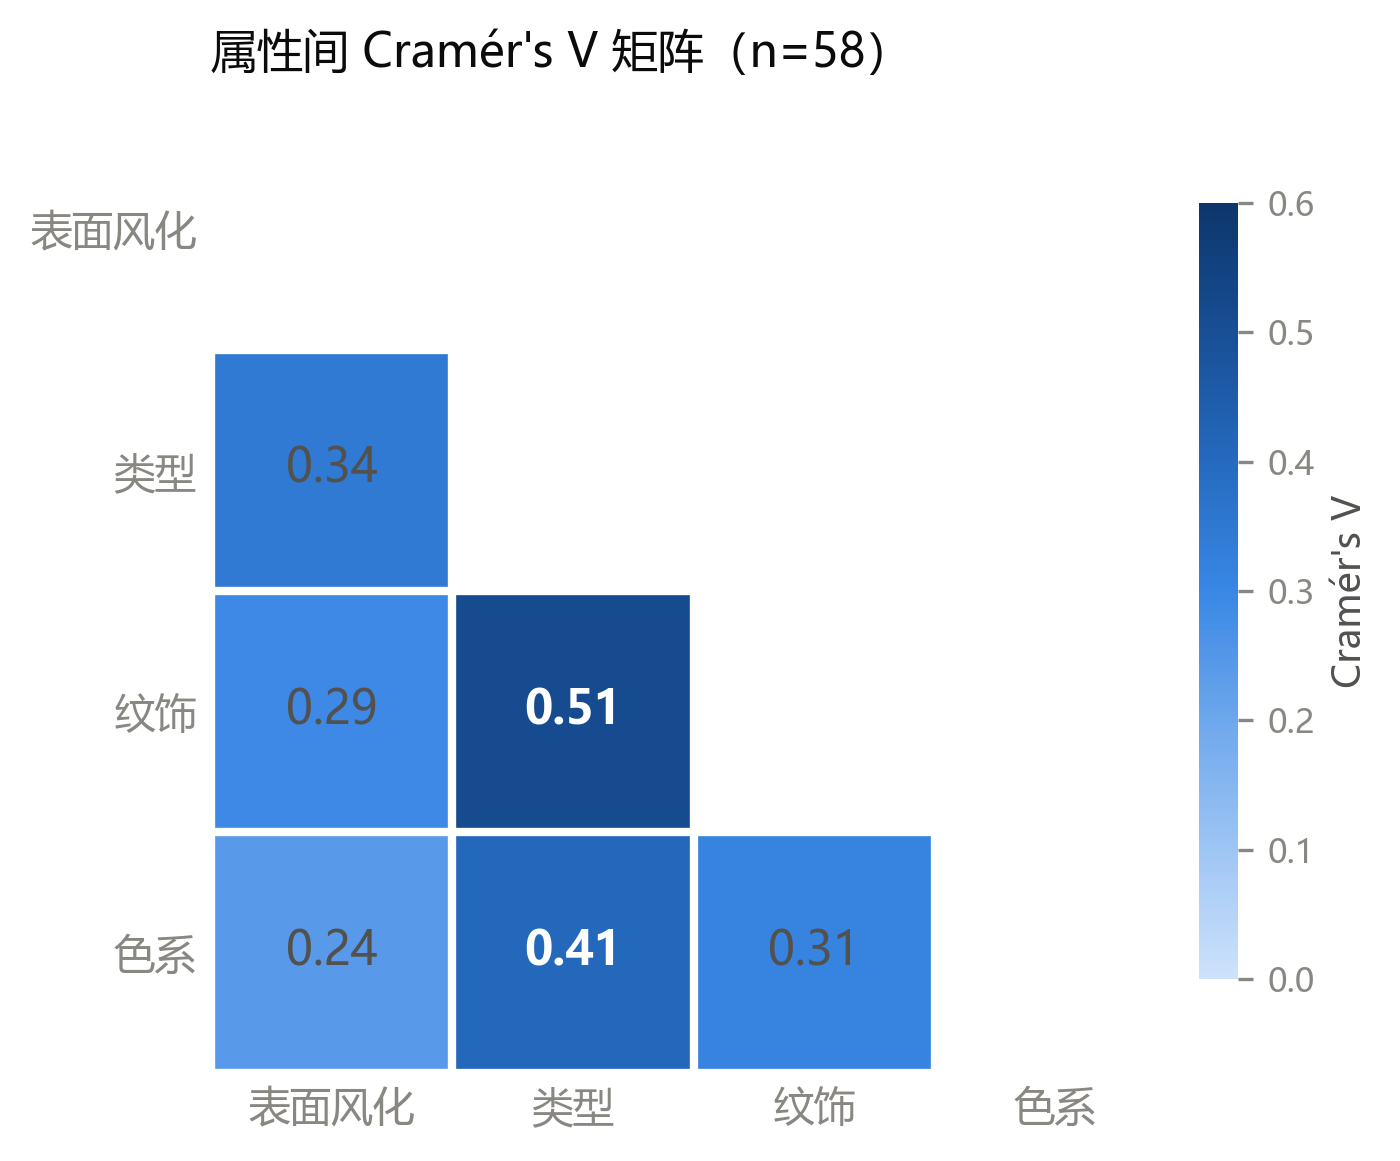
\includegraphics[width=0.62\textwidth]{p1a_fig1_v_heatmap.png}
\caption{四个分类属性之间的 Cramér 关联系数矩阵（下三角，$n=58$）：自变量间的纠缠强于它们与风化的关联}
\label{fig:vheat}
\end{figure}

\subsection{边际关联检验}

\textbf{检验方法的选择。}类型与风化构成 $2\times 2$ 表，主体检验采用 Fisher 精确检验。该表最小期望频数为 7.45，卡方渐近近似在技术上可行，但 Yates 修正与否使 $p$ 值在 0.0087 与 0.0196 之间摆动，小样本下这一口径之争足以动摇结论；Fisher 检验在边缘和固定的条件下精确计算条件分布，不依赖渐近近似，两种卡方口径作为并列证据同时报告。纹饰（$2\times 3$）与色系（$2\times 4$）两表的最小期望频数分别只有 2.48 与 1.66，卡方失效；scipy 未提供 $R\times C$ 的 Fisher--Freeman--Halton 精确检验，故采用固定边缘下的置换检验：在风化与该属性无关的零假设下打乱风化标签 $10^4$ 次，以统计量超过观测值的频率定 $p$ 值。本题 $n=58$ 且类别稀疏，精确或再抽样方法是唯一不引入渐近误差的路线。

\textbf{效应量的不确定性。}$2\times 2$ 表报告优势比及其 Woolf 区间
\begin{equation}
\ln \widehat{OR}\ \pm\ 1.96\sqrt{\sum_{ij}\frac{1}{n_{ij}}}\, ,
\label{eq:orci}
\end{equation}
Cramér 关联系数对全部因素统一计算，并用成对 Bootstrap（$B=5000$）给出百分位置信区间。三对主检验的 $p$ 值经 BH 校正以控制错误发现率。

\begin{table}[htbp]
\centering
\caption{边际筛查汇总（$n=58$；颜色参考行剔除缺失后 $n=54$）}
\label{tab:marginal}
\begin{tabular}{llcccl}
\toprule
因素 & 主检验 & $p$ & $p_{\mathrm{BH}}$ & $V$（95\% CI） & $OR^{a}$ \\
\midrule
类型 & Fisher 精确 & 0.011 & 0.034 & 0.34（$0.09\sim 0.59$） & 4.67（$1.42\sim 15.35$） \\
纹饰 & 置换 $10^4$ & 0.104 & 0.156 & 0.29（$0.18\sim 0.46$） & — \\
色系 & 置换 $10^4$ & 0.363 & 0.363 & 0.24（$0.15\sim 0.45$） & — \\
颜色 8 类$^{b}$ & 置换 $10^4$ & 0.584 & — & 0.34（$0.27\sim 0.59$） & — \\
\bottomrule
\multicolumn{6}{l}{\footnotesize $^{a}$ 铅钡相对高钾的风化优势比。$^{b}$ 参考行，类别过稀，不参与 BH 校正。}\\
\multicolumn{6}{l}{\footnotesize 类型行的并列证据：未校正 $\chi^2=6.88$（$p=0.0087$），Yates $\chi^2=5.45$（$p=0.020$）。}\\
\end{tabular}
\end{table}

\begin{figure}[htbp]
\centering
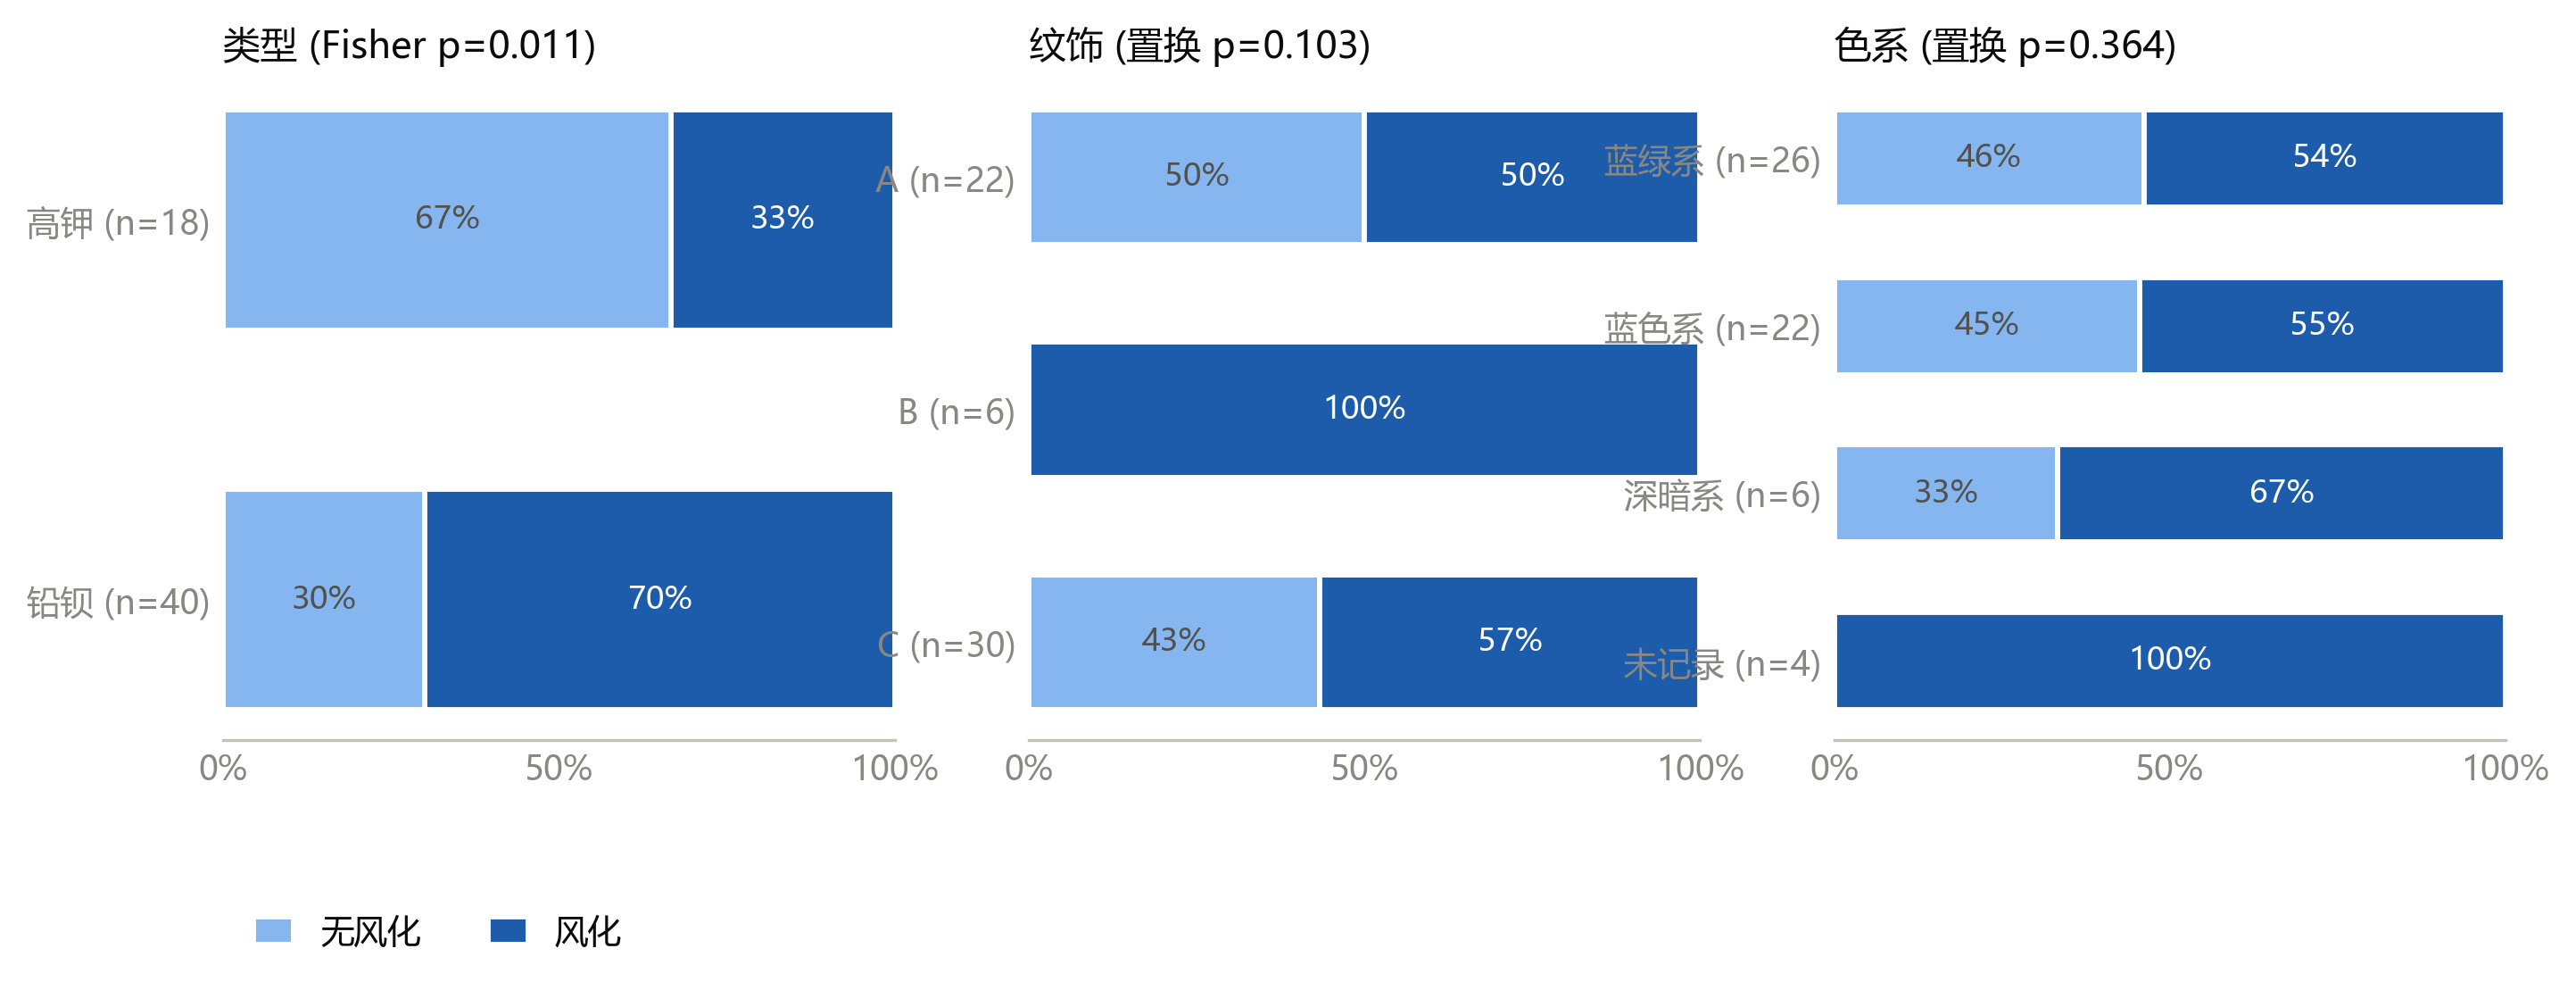
\includegraphics[width=0.98\textwidth]{p1a_fig3_wxrate_bars.png}
\caption{各属性内部的风化占比：类型两档相差 37 个百分点，纹饰 B 档 6 件全部风化，色系各档差异平缓}
\label{fig:rate}
\end{figure}

\begin{figure}[htbp]
\centering
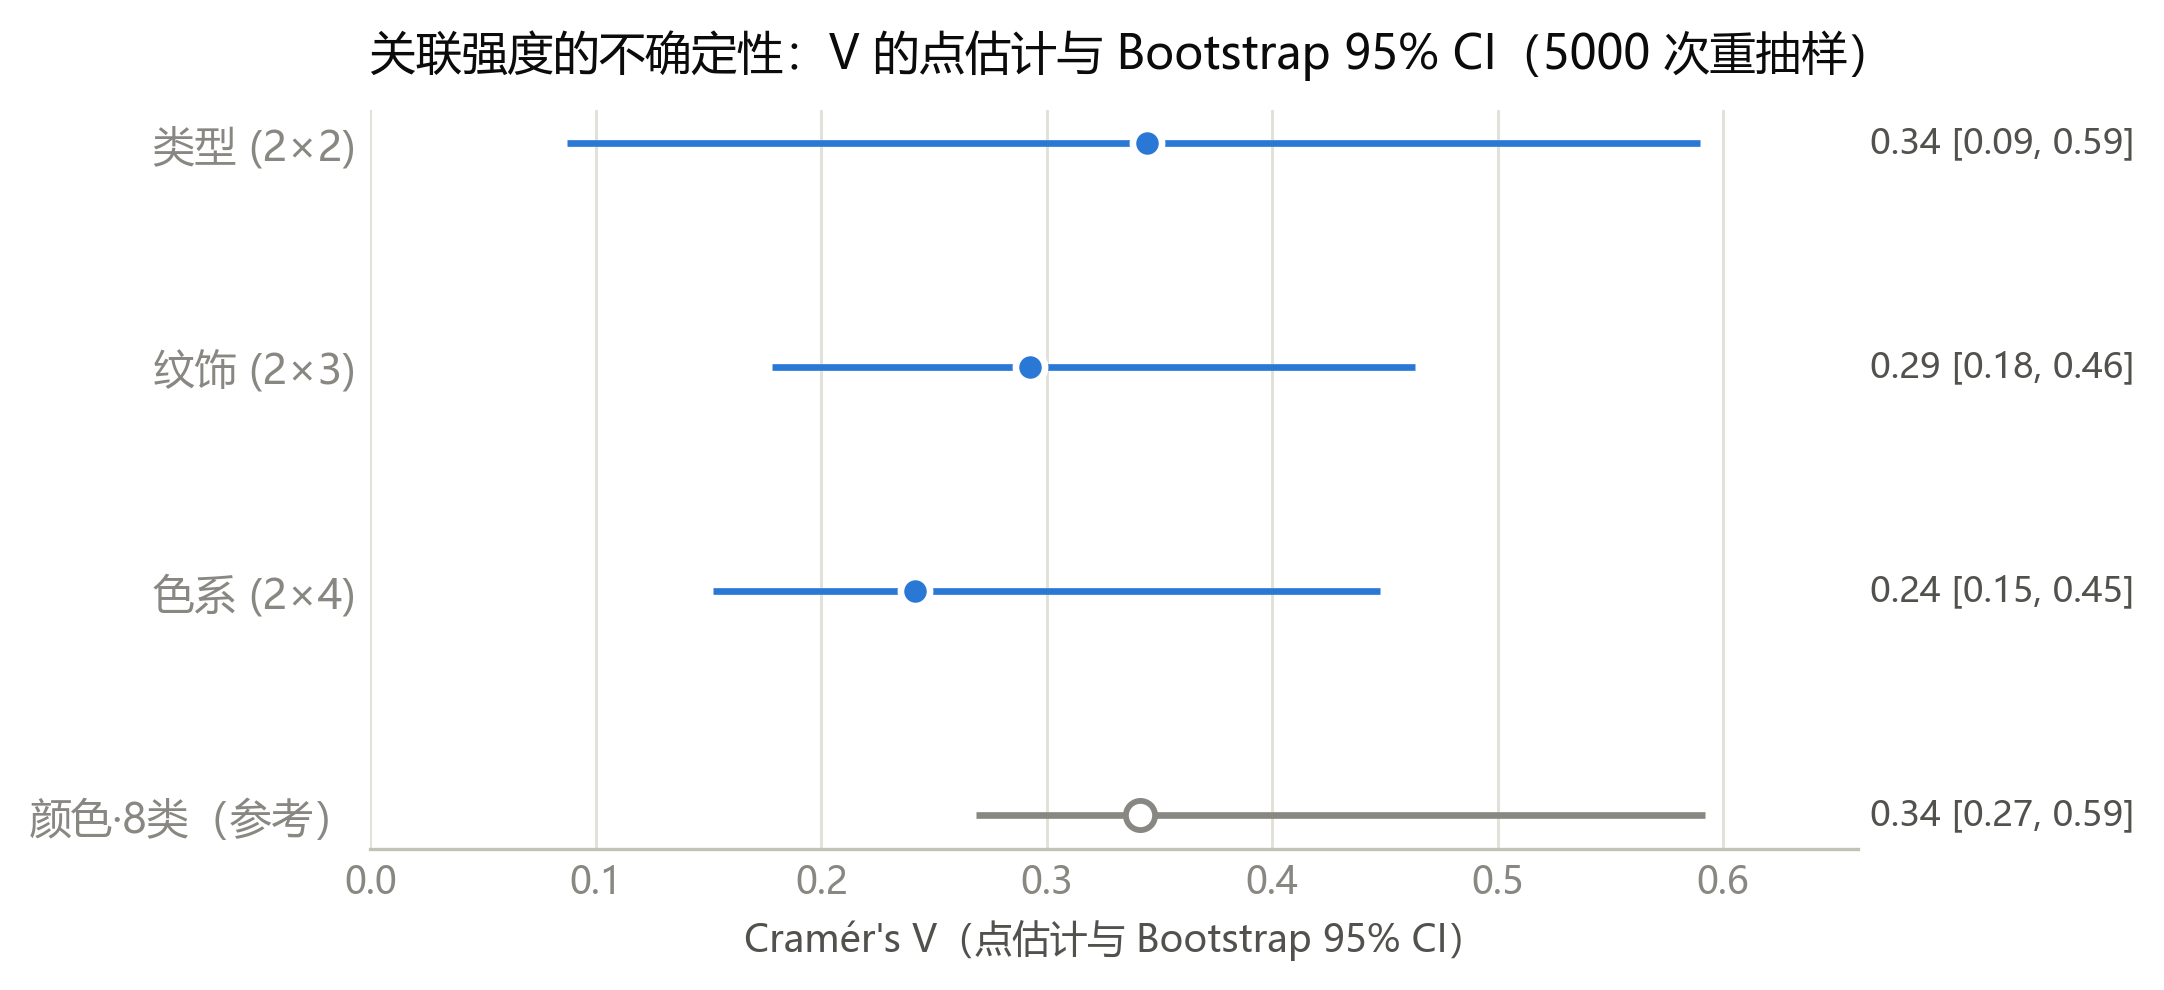
\includegraphics[width=0.9\textwidth]{p1a_fig2_v_forest.png}
\caption{关联强度的不确定性：$V$ 的点估计与 Bootstrap 95\% CI（$B=5000$），三个主因素区间全部重叠，颜色 8 类（空心点）为参考}
\label{fig:vforest}
\end{figure}

结果见表~\ref{tab:marginal} 与图~\ref{fig:rate}、图~\ref{fig:vforest}。类型与风化的关联显著：风化率在高钾为 33.3\%（6/18）、铅钡为 70.0\%（28/40），Fisher $p=0.011$，铅钡的风化几率是高钾的 4.67 倍（95\% CI $1.42\sim 15.35$），$\varphi=0.34$；BH 校正后 $p=0.034$，是唯一通过 0.05 门槛的因素。纹饰（$p=0.104$）与色系（$p=0.363$）均不显著。图~\ref{fig:vforest} 显示三个因素的 Bootstrap 区间大面积重叠，其中颜色 8 类的 $V$ 点估计 0.341 与 $p=0.584$ 并存：类别过稀把 $V$ 抬高，Bootstrap 中位数 0.430 高于点估计，这正是裸 $V$ 不可直接排序的实证。据此本节只做类型显著、其余无信号的保守表述，不做最强因素的排名。

边际筛查留下两处待解释的痕迹。其一，纹饰三档的风化率呈 A 50.0\%、B 100.0\%、C 56.7\% 的结构，B 的 6 件全部风化但边际检验不显著；其二，纹饰与类型的关联达 $V=0.51$，B 的信号可能与类型纠缠。两者的裁决交给下一节的分层分析。

\subsection{按类型分层的纹饰与颜色分析}

回答纠缠问题最直接的办法是分层：把 58 件文物按类型分成铅钡层（40 件）与高钾层（18 件），在每层内部重新考察纹饰、色系与风化的关系。若纹饰的信号完全由类型传导，层内对比应当归于平淡；若层内仍然极端，则说明存在类型之外的独立结构。这一做法不引入任何新模型，代价是层内样本量更小，因此检验全部沿用精确或置换口径。

\begin{table}[htbp]
\centering
\caption{按类型分层后各纹饰档的风化计数与风化率}
\label{tab:strat}
\begin{tabular}{llcccc}
\toprule
层 & 纹饰档 & $n$ & 无风化 & 风化 & 风化率 \\
\midrule
铅钡（40 件） & A & 16 & 5 & 11 & 68.8\% \\
铅钡（40 件） & C & 24 & 7 & 17 & 70.8\% \\
高钾（18 件） & A & 6 & 6 & 0 & 0\% \\
高钾（18 件） & B & 6 & 0 & 6 & 100\% \\
高钾（18 件） & C & 6 & 6 & 0 & 0\% \\
\bottomrule
\multicolumn{6}{l}{\footnotesize 铅钡层内 A 与 C 的 Fisher $p=1.00$；B 档无铅钡样本。}\\
\multicolumn{6}{l}{\footnotesize 高钾层的组合概率与层内置换 $p$ 值见正文。}\\
\end{tabular}
\end{table}

\begin{figure}[htbp]
\centering
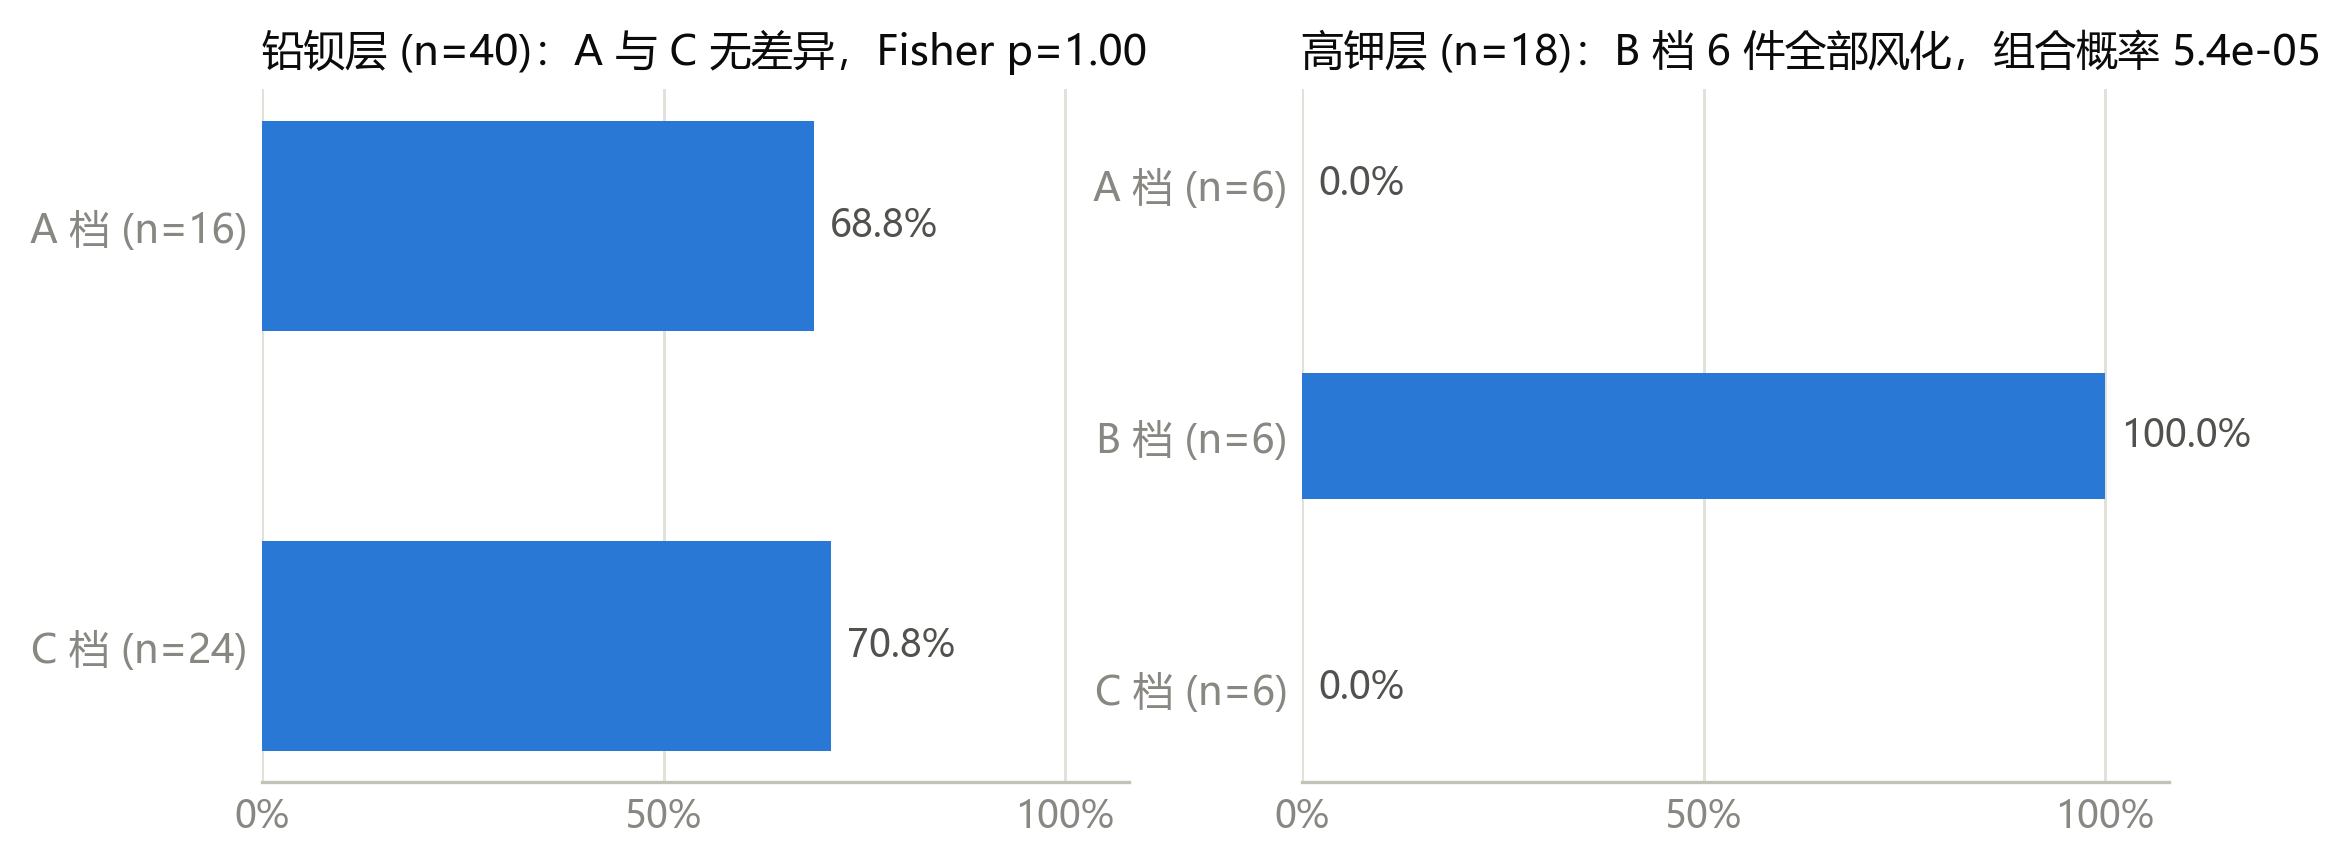
\includegraphics[width=0.94\textwidth]{p1a_fig4_stratified.png}
\caption{按类型分层后各纹饰档的风化率：铅钡层内 A、C 两档无差异，高钾层内 B 档 6 件全部风化、A 与 C 档 12 件全部无风化}
\label{fig:strat}
\end{figure}

表~\ref{tab:strat} 与图~\ref{fig:strat} 给出分层结果。铅钡层内纹饰与风化无关：A 档 16 件中风化 11 件（68.8\%），C 档 24 件中风化 17 件（70.8\%），Fisher $p=1.00$。高钾层内则出现极端结构：风化的 6 件全部是 B 档，A 档与 C 档的 12 件全部无风化。若高钾层内风化与纹饰无关，6 件风化文物恰好全部落入 B 档 6 个槽位的组合概率为
\[
\frac{1}{\binom{18}{6}}=5.4\times 10^{-5},
\]
以层内卡方为统计量、在高钾层内打乱风化标签 $10^4$ 次的层内置换检验给出 $p=0.0001$。两个口径一致指向同一结论：给定类型之后，纹饰 B 档与风化完全对应。对照其边际检验的 $p=0.104$，纹饰的信号在边际层面被类型完全掩蔽，分层后现出原形。

色系的分层检验同样不支持独立关联：铅钡层内置换 $p=0.594$；高钾层内深暗系没有样本，蓝绿系与蓝色系之间的 Fisher $p=0.114$。边际筛查中色系无信号的判断在分层后保持不变。

作为复核，我们以 Firth 惩罚逻辑回归将三属性同时入模：普通逻辑回归因纹饰 B 的完全分离无法估计（迭代发散，$\max|\beta|=68.6$），Firth 惩罚估计给出类型的调整后 $OR=0.021$（$0.001\sim 0.383$），与分层结论一致；纹饰 B 的系数则因分离只能给出跨四个数量级的宽区间，故本文不把该模型列为主线证据。

\subsection{单变量与联合分析的对照}

前两节实际完成了同一问题的两套分析：1.5 节把每个属性单独与风化比较，1.6 节把类型作为分层变量纳入后再看纹饰与色系。两套结果的并排对照见表~\ref{tab:contrast}，联合考虑的收益在其中表现为三种可数值化的性质。

\begin{table}[htbp]
\centering
\caption{单变量分析与分层联合分析的结论对照}
\label{tab:contrast}
\footnotesize
\begin{tabular}{p{1.2cm}p{3.9cm}p{4.6cm}p{3.6cm}}
\toprule
属性 & 单独考虑（1.5 节） & 联合考虑（1.6 节分层） & 性质差异 \\
\midrule
类型 & Fisher $p=0.011$，$OR=4.67$（$1.42\sim 15.35$），判相关 & 背景主效应；Firth 复核调整后 $OR=0.021$（$0.001\sim 0.383$） & 同向，复核排除纹饰 B 档混杂对效应量的压缩 \\
纹饰 & 置换 $p=0.104$，判无关 & 铅钡层 Fisher $p=1.00$；高钾层组合概率 $5.4\times 10^{-5}$、层内置换 $p=0.0001$ & 假阴性纠正：单变量漏检的强信号被检出 \\
色系 & 置换 $p=0.363$，但 $V=0.341$ 虚高 & 铅钡层 $p=0.594$；高钾层 $p=0.114$ & 虚高线索被排除：确认无独立关联 \\
颜色 8 类 & $V=0.341$ 与 $p=0.584$ 并存 & 参考行，不参与分层检验 & 稀疏假象被识别 \\
\bottomrule
\end{tabular}
\end{table}

表~\ref{tab:contrast} 的对照给出三点收益，均有数值支撑。其一，判断的对错：单独考虑对纹饰判无关，实为高钾层内的强关联，假阴性由分层证据纠正，纠正后的结论有组合概率与层内置换两重独立口径支撑。其二，效应量的精度：类型的表观 $OR=4.67$ 混有纹饰 B 档的压缩作用，Firth 复核值 0.021 与表观值 4.67 之间的落差本身就是混杂强度的度量。其三，排名的可靠性：单独考虑时颜色的 $V=0.341$ 在三个因素中名列第二，联合后确认其无独立贡献，直接以裸 $V$ 排名将误导后续特征筛选。三项归纳为一句话：单独考虑的三项主结论中一项判错、一项伴随虚高效应量，联合考虑后全部归位。

\subsection{求解环境与稳健性}

求解环境为 Python 3.14.3，numpy 2.4.3、pandas 3.0.1、scipy 1.17.1、matplotlib 3.10.8；Bootstrap 5000 次、置换 $10^4$ 次，随机种子 2026 固定，全流程耗时约 0.4 min。置换次数的依据：$p$ 值在 0.01 量级时，$10^4$ 次置换的蒙特卡洛标准误约为 $10^{-3}$，足以分辨本文涉及的显著性水平。

稳健性从四个方向检查。第一，卡方口径：类型检验的未校正 $p=0.0087$ 与 Yates 修正 $p=0.020$ 并列报告，两者与 Fisher 的 0.011 结论一致。第二，多重比较：BH 校正后类型 $p=0.034$ 仍为唯一过线因素，结论集不变。第三，缺失口径：剔除颜色未记录的 4 件后，类型 Fisher $p=0.041$（全样本 0.011），纹饰置换 $p=0.057$，色系 $p=0.861$；类型关联在两种口径下均过 0.05 门槛，但 $p$ 值对这 4 件的取舍敏感，提示其边际关联强度中等，结论以分层结构与 1.6 节的 Firth 复核为凭。第四，不确定性：图~\ref{fig:vforest} 中三个主因素的 Bootstrap 区间全部重叠，本文不做任何最强因素的排名宣称。

\subsection{小结}

\begin{enumerate}
\item 类型与风化存在独立关联。风化率在高钾为 33.3\%、铅钡为 70.0\%，边际 $OR=4.67$（95\% CI $1.42\sim 15.35$），Fisher $p=0.011$；分层分析与 Firth 复核（调整后 $OR=0.021$，$0.001\sim 0.383$）均支持该结论。
\item 纹饰 B 的信号在分层后显现。铅钡层内 A、C 两档风化率 68.8\% 对 70.8\%（Fisher $p=1.00$）；高钾层内 6 件风化全部为 B 档（组合概率 $5.4\times 10^{-5}$，层内置换 $p=0.0001$），而边际检验 $p=0.104$ 掩蔽了该信号。
\item 颜色无独立贡献。边际置换 $p=0.363$，分层后铅钡层 $p=0.594$、高钾层 $p=0.114$；颜色缺失的 4 件全部为风化铅钡，按未记录类单列处理。
\item 边际分析在本数据上同时产生两类错误：对纹饰产生假阴性（0.104 对 0.0001），对颜色保留虚高线索（$V=0.341$ 对 $p=0.584$）。分层框架将两者同时纠正（对照见表~\ref{tab:contrast}），这是联合考虑的直接收益。
\item 结论的失效边界：纹饰 B 的发现基于 6 件样本且属事后分析，只能作为待检验线索；全部结论限于本批 58 件样本，外推需更大样本。该联合结构同时要求问题一后半的风化规律分析与成分回推按类型分层进行。
\end{enumerate}

% ------------------------------------------------------------------
% AI 工具使用声明（2026 新规要求，正式提交时置于参考文献之前）：
% 本节初稿由 Claude（Claude Code，模型 claude-fable-5）辅助起草，
% 统计计算由随附脚本 p1a_main.py 完成（随机种子 2026，可复现），
% 作者对全部数值与结论进行了核对。按竞赛要求另附《AI工具使用详情.pdf》。
% ------------------------------------------------------------------

\end{document}
